\chapter{Introduction}
\label{chapter1}
\section{Context}
The signed distance field (SDF) is a solution for solving boundary problems. The research of SDF in Computer Graphics, especially for 3D shapes representation, has developed \cite{SDFSurvey}. For example, collision detection \cite{RigidDetec} \cite{SoftDetec}, liquid simulation \cite{liquid} and ray-marching \cite{hart1996sphere}. In recent years, related research results have been applied in the industry, for example, the Unreal Engine \cite{uesdf}.

\section{Project Aim}

The main aim of this project is to build a tool to generate a signed distance field (SDF) for three-dimensional objects and implement a suitable SDF generate algorithm. The tool is expected to visualize the SDF calculate result as well.

\section{Objectives}

\begin{itemize}
    \item Build a application that can read in and visualize given triangular meshes.
    \item Implement a SDF generating algorithm.
    \item Build a application to visualize the SDF compute result
    \item Comment the code properly for potential reuse
    \item Test the tool on multiple devices
\end{itemize}

\section{Deliverables}

\begin{itemize}
    \item A application that generate Signed Distance Field.
    \item A GitHub repository that contains the source code of the tool.
    \item The MSc project report
\end{itemize}

\clearpage

\section{Project Plan}

The project will be implemented through the waterfall model as it has precise requirements and is easy to implement \cite{balaji2012waterfall}. Every new feature will be implemented after the last phase is completely finished. The first phase is research and design. It takes four months to ensure that this project's requirement is rational and realistic. The programming work starts from the middle of June to early August. Most time is assigned to algorithm implementation, and then most time will be used to evaluate and write the report.

\hspace*{\fill}

The Gannt chart of time management for this project is shown in figure \ref{inro:gannt}.

\begin{figure}[htbp]
    \centering
    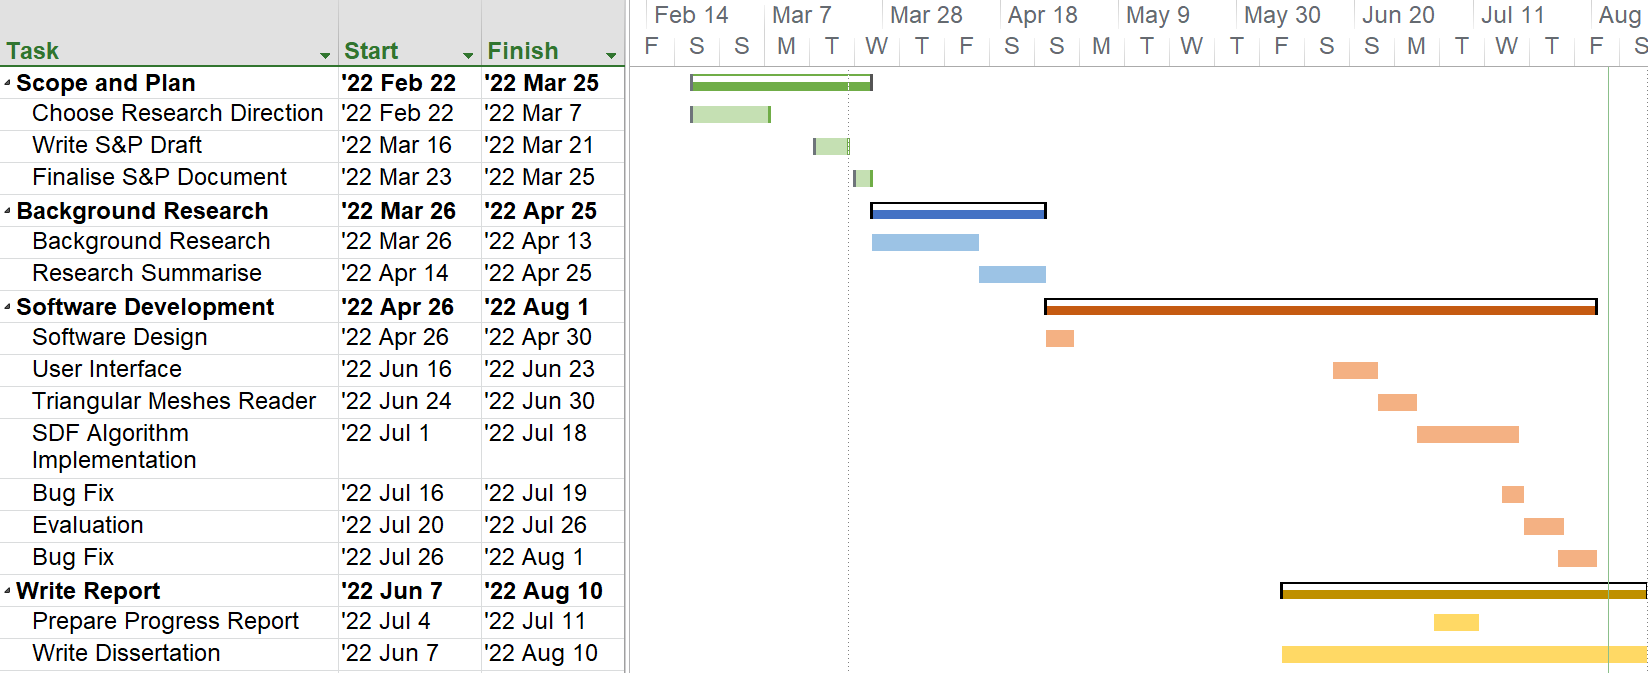
\includegraphics[width=16cm]{Images/Chap1/Gannt.png}
    \caption{The time management Gannt chart}
    \label{inro:gannt}
\end{figure}

\section{Report Structure}
This report is divided into six chapters.

\hspace*{\fill}

The first chapter introduces the project aims and objectives and discusses potential ethical, legal and social issues. The second one presents the background research for the project, including a survey of past SDF-related research and the methodology and technologies used in the project. The third chapter documents the design of the software product, while the fourth one is about detailed implementation. The contents of chapter five illustrate the test and evaluation results. Finally, the conclusion and potential improvements can be found in the sixth chapter.

\clearpage

\section{Ethical, legal, and social issues}

The SDF generate software product of this project only reads in and processes triangular meshes; it does not collect personal data at any time. Therefore, there are no significant ethical or social issues.

\hspace*{\fill}

Several open source third-party libraries have been contained and invoked in the source code to save development time and use test data sets quickly. All usage of the libraries followed its licenses to avoid potential plagiarism and legal issues.